
\newpage

\section{File Inclusion}

De nombreux langages de programmation permettent d'inclure des portions de code contenues dans d'autres fichiers que celui en cours d'exécution. Le mécanisme mis à disposition permet de recopier dans le script principal le code contenu dans un autre fichier. Cette procédure est transparente à l'œil de l'utilisateur et peut être très avantageuse pour le développeur d'un site internet.

\begin{figure}[!h]
\begin{center}

\label{inclusion}
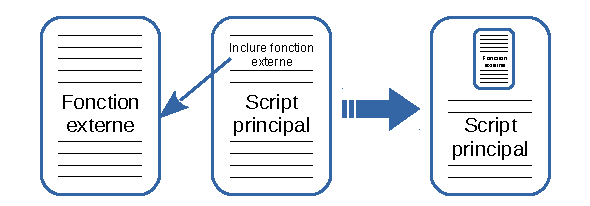
\includegraphics[scale=1.2]{images/include.pdf}

\caption{Mécanisme d'inclusion d'un fichier}

\end{center}
\end{figure}

En effet, inclure du code contenu dans un autre fichier permet, entre autre, les deux utilisations suivantes :
\begin{itemize}
\item inclure des portions de code différentes en fonction de choix de l'utilisateur ou de l'environnement de ce dernier;
\item inclure des portions de code utilisées dans plusieurs scripts (par exemple une fonction de connexion à une base de données) afin de ne pas avoir à recopier les mêmes lignes à différents endroits et de ne modifier qu'un seul fichier en cas de modification de la fonction.
\end{itemize}





\subsection{Description de la vulnérabilité}

La principale vulnérabilité connue dans le mécanisme que nous venons d'expliciter intervient lorsque l'inclusion d'un script est gérée par une variable pouvant être contrôlée par un attaquant. On se retrouve alors plutôt dans le premier cas d'utilisation indiqué, c'est à dire inclure des portions de code différentes en fonction de choix de l'utilisateur ou de l'environnement de ce dernier. En effet, dans le second cas d'utilisation, l'inclusion du fichier est généralement écrite "en dur" dans le script principal et ne peut donc pas être facilement modifiée par un attaquant.

\begin{figure}[!h]
\begin{center}

\label{inclusion_hacked}
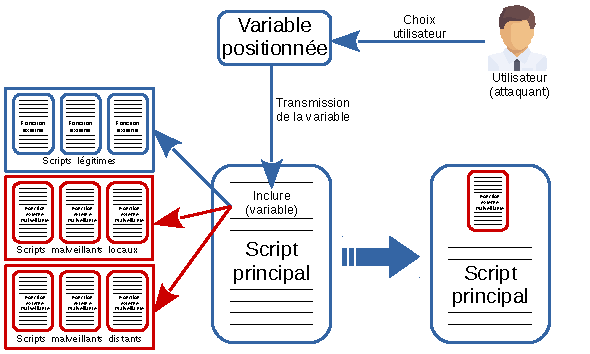
\includegraphics[scale=1.4]{images/include_hacked.pdf}

\caption{Vulnérabilité d'inclusion d'un fichier}

\end{center}
\end{figure}

On remarque dans le schéma \ref{inclusion_hacked} que dans le cas où un attaquant peut avoir accès à la variable permettant de sélectionner le script légitime, celui-ci peut en modifier le contenu de deux façons. On parle alors de Local File Inclusion (LFI) et de Remote File Inclusion (RFI).

\subsubsection{Local File Inclusion}

Une fois que l'attaquant est en capacité de modifier le contenu de la variable indiquant le nom du script à inclure, celui-ci peut y indiquer un chemin local (i.e. directement sur le serveur) vers un script contenant du code malveillant. Il peut s'agir d'un script que l'attaquant a au préalable placé sur le serveur ou d'un script déjà présent qui effectue des opérations pouvant porter atteinte à la disponibilité de la machine voire à l'intégrité ou la confidentialité des données.

\subsubsection{Remote File Inclusion}

L'attaquant peut également indiquer dans la variable un chemin distant (i.e. vers un autre serveur) pointant vers un script contenant du code malveillant. Cette technique a pour avantage de faciliter la gestion du contenu du script malveillant par l'attaquant qui peut y inclure toutes les fonctionnalités qu'il souhaite voire le faire évoluer en fonction de la réponse de la machine attaquée.\\

Dans les deux cas, les scripts malveillants sont recopiés au sein du code du script principal qui sera au final exécuté par le serveur. Cette vulnérabilité offre donc de vastes possibilités à un attaquant qui peut alors faire exécuter par un serveur n'importe quelles fonctionnalités qu'il souhaite.

\subsection{Exploitation de la vulnérabilité}

\subsection{Contre-mesure}

\section{File Upload}

De très nombreuses applications web laissent la possibilité à l'utilisateur de charger des fichiers qu'il détient en local sur son propre ordinateur. On peut bien entendu citer à ce titre les serveurs de messagerie électronique ainsi que les clients web permettant la gestion d'un \textit{cloud}. En effet, sans cette fonctionnalité de chargement, il serait impossible de joindre un fichier à mail ou même de sauvegarder ses fichiers dans le \textit{cloud}. 

Nous allons voir que cette fonctionnalité doit être bien encadrée et supervisée afin de ne pas créer de très importantes vulnérabilités.

\subsection{Description de la vulnérabilité}

\subsubsection{Généralités}

Le chargement d'un fichier local vers un serveur web est une fonctionnalité nécessaire voire inhérente à certaines applications web. Sans cette possibilité, certaines applications n'auraient même pas de raison d'être. Ainsi, \textit{Gmail}, \textit{Google Drive} ou \textit{DropBox} reposent sur cette possibilité. Il est donc nécessaire de trouver le moyen de faire face aux différentes vulnérabilités de cette fonction.

Un grand nombre d'attaques sur les applications web se déroulent en deux phases :
\begin{enumerate}
\item injection d'un code malicieux sur le serveur web;
\item exécution du code malicieux précédemment injecté.
\end{enumerate} 
On peut donc clairement voir que le chargement d'un fichier local vers un serveur web offre une possibilité claire à un attaquant de charger sur le serveur web un fichier contenant du code malicieux. Il ne lui restera alors plus qu'à trouver un moyen d'exécuter ce code.

De plus, il est à noter que n'importe quel type de script peut, grâce à cette fonction, être importé sur le serveur web. Cela laisse donc la porte ouverte à un grand nombre d'attaques différentes : déni de service, défacement, prise en main du système, etc...

Afin de retirer ces possibilités d'action à un attaquant éventuel, il sera alors nécessaire de restreindre le chargement à certains types de fichiers ou d'effectuer certains contrôles.

\subsubsection{Différentes vulnérabilités}

La plateforme \href{http://www.owasp.org}{OWASP} classe les vulnérabilités liées au chargement de fichiers en deux catégories : les vulnérabilités liées aux méta-données et les vulnérabilités liées à la taille ou au type des fichier.

\paragraph{Les vulnérabilités liées aux méta-données :}

Ces vulnérabilités sont dues aux différents champs échangés dans les requêtes HTTP, principalement le champ indiquant le chemin de destination du fichier ainsi que le champ indiquant le nom du fichier.

En effet, en modifiant les champs des requêtes HTTP multi-part (utilisées dans le chargement et le téléchargement de fichiers sur un serveur web), il est possible d'écraser des fichiers déjà existants ou même d'atteindre des répertoires normalement non autorisés à l'écriture par un utilisateur.

Cette classe de vulnérabilités permet donc par exemple d'effectuer un défacement, d'insérer du code malicieux dans des dossiers stratégiques ou encore de modifier le comportement normal d'un script.

\paragraph{Les vulnérabilités liées à la taille ou au type des fichiers :}

Ces vulnérabilités sont principalement dues à l'absence de certaines vérifications avant le début du chargement du fichier. 

Ainsi, la non vérification de la taille d'un fichier laisse la possibilité aux utilisateurs de charger des fichiers aussi volumineux qu'ils le souhaitent. Il est alors possible sur certains serveurs dont l'espace de stockage est limité d'atteindre la capacité maximale de cet espace et, par là, de rendre la fonctionnalité de chargement voire le serveur lui-même indisponible. On peut donc aboutir très rapidement à une attaque du type déni de service.

De même, la non-vérification du type de fichier peut permettre à un utilisateur de charger sur le serveur un script exécutable alors que le fichier attendu était par exemple une photographie. Un tel script pourra alors être \textit{a posteriori} exécuté par l'attaquant lui donnant ainsi de nombreuses possibilités.\\

On voit donc que le chargement de fichier sur un serveur web est loin d'être anodin et doit être encadré afin d'éviter qu'un utilisateur ait à sa disposition un large éventail d'attaques possibles.


\subsection{Exploitation de la vulnérabilité}

\subsection{Contre-mesure}

\section{Insecure CAPTCHA}

De nombreux robots (ou \textit{bots}) agissent de façon automatique sur internet afin, principalement, d'envoyer des messages, qu'ils soient publicitaires ou malveillants. La plupart des spams échangés sur internet sont d'ailleurs le fait de tels robots. Il est donc nécessaire, dans certaines applications web permettant notamment l'envoi de messages, de vérifier s'il s'agit d'un humain ou d'une machine qui souhaite effectuer cette opération.

C'est dans ce but que les contrôles CAPTCHA ont été créés. En effet, CAPTCHA est l'acronyme de \textit{Completely Automated Public Turing test to tell Computers and Human Apart}. Comme son nom l'indique, ce test est censé permettre de confirmer ou non la présence d'un humain derrière la machine souhaitant réaliser une certaine opération. Ce test peut prendre plusieurs formes : reconnaissance de caractères déformés ou encore reconnaissance d'éléments dans un puzzle.

Pour que ce test soit efficace, il est nécessaire qu'il soit implémenté de façon correcte et, ainsi, ne pas laisser la possibilité à un attaquant d'exploiter une faille qu'il pourra par la suite réutiliser dans un script automatique.
 

\subsection{Description de la vulnérabilité}

Différentes catégories de vulnérabilités peuvent être mises en évidence concernant les contrôles CAPTCHA.

\paragraph{Transmission de la solution :}

La première et la plus simple à exploiter est lorsque la solution se trouve être transmise en texte clair au navigateur client. Il ne suffit que de repérer l'endroit où se trouve la solution pour réaliser un script qui résoudra à coup sûr chaque contrôle CAPTCHA. En effet, les solutions peuvent être passées en argument de l'URL, dans le nom de l'image, dans un champ caché d'un formulaire HTML ou encore en commentaire du fichier HTML chargé. 

\paragraph{Mauvaise vérification de la réussite au test :}

La deuxième catégorie de vulnérabilités concerne le fait que le contrôle CAPTCHA peut être outrepassé si la vérification de la réussite au test n'est pas suffisamment sécurisée. En effet, la ou les variables indiquant une réussite ou non au test doivent être protégées et ne pas être facilement modifiées sans avoir à réaliser le test au préalable. Dans le cas contraire, il est encore possible de trouver une parade à la réalisation du test par un humain et de l'implémenter dans un script automatique.

\paragraph{Résolution automatique :}

Enfin, la troisième catégorie de vulnérabilités concerne la possibilité de résoudre de façon automatique les contrôles CAPTCHA. Dans cette catégorie, beaucoup de problèmes sont à prendre en compte : la difficulté du problème, le temps de résolution du problème ou encore l'étendue de la base de données CAPTCHA. En effet, ce dernier point est important car si la base de données d'images par exemple n'est pas assez grande, une entité pourrait facilement trouver un avantage financier à payer des personnes pour résoudre tous les problèmes CAPTCHA afin de pouvoir les exploiter automatiquement par la suite.

\subsection{Exploitation de la vulnérabilité}

\subsection{Contre-mesure}








